%
% Complete documentation on the extended LaTeX markup used for Insight
% documentation is available in ``Documenting Insight'', which is part
% of the standard documentation for Insight.  It may be found online
% at:
%
%     http://www.itk.org/

\documentclass{InsightArticle}

\usepackage[dvips]{graphicx}

%%%%%%%%%%%%%%%%%%%%%%%%%%%%%%%%%%%%%%%%%%%%%%%%%%%%%%%%%%%%%%%%%%
%
%  hyperref should be the last package to be loaded.
%
%%%%%%%%%%%%%%%%%%%%%%%%%%%%%%%%%%%%%%%%%%%%%%%%%%%%%%%%%%%%%%%%%%
\usepackage[dvips,
bookmarks,
bookmarksopen,
backref,
colorlinks,linkcolor={blue},citecolor={blue},urlcolor={blue},
]{hyperref}


%  This is a template for Papers to the Insight Journal.
%  It is comparable to a technical report format.

% The title should be descriptive enough for people to be able to find
% the relevant document.
\title{Conformal Flattening ITK Filter}

% Increment the release number whenever significant changes are made.
% The author and/or editor can define 'significant' however they like.
\release{0.00}

% At minimum, give your name and an email address.  You can include a
% snail-mail address if you like.
\author{Yi Gao$^{1}$ and et al $^{1}$ $^{2}$ $^{3}$}
\authoraddress{$^{1}$Georgia Institute of Technology, Atlanta, GA\\
               $^{2}$Kitware, Clifton Park, NY\\
               $^{3}$GE, Niskayuna, NY}

\begin{document}

\newif\ifpdf
\ifx\pdfoutput\undefined
  \pdffalse
\else
  \pdfoutput=1
  \pdftrue
\fi


\ifpdf
\else
   %
   % Commands for including Graphics when using latex
   %
   \DeclareGraphicsExtensions{.eps,.jpg,.gif,.tiff,.bmp,.png}
   \DeclareGraphicsRule{.jpg}{eps}{.jpg.bb}{`convert #1 eps:-}
   \DeclareGraphicsRule{.gif}{eps}{.gif.bb}{`convert #1 eps:-}
   \DeclareGraphicsRule{.tiff}{eps}{.tiff.bb}{`convert #1 eps:-}
   \DeclareGraphicsRule{.bmp}{eps}{.bmp.bb}{`convert #1 eps:-}
   \DeclareGraphicsRule{.png}{eps}{.png.bb}{`convert #1 eps:-}
\fi


\maketitle


\ifhtml
\chapter*{Front Matter\label{front}}
\fi


% The abstract should be a paragraph or two long, and describe the
% scope of the document.
\begin{abstract}
\noindent This document describes the Insight Toolkit (ITK)
Conformal Flattening filter.
\end{abstract}

\tableofcontents

Here we provide background on Conformal Flattening (angle
preserving, literature review, practical uses such as brain
flattening).

\section{Algorithm Details}

\subsection{The central goal of the paper}
  The original surface $\Sigma$, a 3-d point set, is given by $P_i(x,
  y, z)$.

  The goal is to map those points onto a plane, and then onto a
  sphere.  The mapping should have some properties, like angle
  preserving in this case.

  So:

  \begin{displaymath}
    \Sigma \qquad \rightarrow \qquad plane \rightarrow  \qquad sphere
  \end{displaymath}

  The first arrow above is achieved by the conformal mapping while the
  second is by the stereographic projection.

  It is shown in the appendix that the conformal mapping is the
  function $z$ defined by equation:

  \begin{eqnarray}
    \triangle z = (\frac{\partial}{\partial u} -
    i\frac{\partial}{\partial v})\delta_p \label{pde}
  \end{eqnarray}
  where $p$ is an (arbitrary) point on $\Sigma$. Through this mapping
  $z$, we map $\Sigma \backslash \{ p \}$ to complex plane \emph{C}.


  \subsection{How to get the mapping function $z$}
  So the problem turns out to be: how to solve the mapping function
  $z$ from the equation \ref{pde}.

  $z$ solve equation \ref{pde} iff $\forall$ smooth function f:

  \begin{eqnarray}
    \int\int_{\Sigma}\nabla z \cdot \nabla f \textrm{d}S =
    (\frac{\partial f}{\partial u} - i\frac{\partial f}{\partial
      v})|_p \label{inteqn}
  \end{eqnarray}  

  Next, we have to calculate both sides of equation \ref{inteqn} on
  the discrete mesh.

  \begin{enumerate}
  \item \emph{The right side} The right side is basically ZERO
    except on those THREE points in which the point $p$ (of the Dirac
    function) lies. For those three points, A, B, C, the right side of
    equation \ref{inteqn} is:
    \begin{eqnarray}
      \frac{f_A - f_B}{|| B - A ||} + i\frac{f_c-(f_A + \theta(f_B -
        f_A))}{||C - E||} \label{Rinteqn}
    \end{eqnarray}  
    where the point E is the point D in the derivation at the right
    bottom of page 701 of the paper. In the later part of the paper this
    point is refered to as E so I use E here.

    With this, the right side of equation \ref{inteqn} is solved.

  \item \emph{The left side} We use a piecewise linear function
    defined on $\Sigma$ to approximate the function f. Because the
    $\Sigma$ is a discrete mesh, let N be the total number of points
    in the mesh. Hence, the piecewise linear function space on the
    mesh is only N-dimensional. Define the basis to be, $\Phi_i$, as in the
    paper. Then we can write function z as $z = \sum_{k=1}^{N}z_k
    \Phi_k$

    So equation \ref{inteqn} becomes:
    \begin{eqnarray}
      \sum_{P}z_P \int\int (\nabla \Phi(P) \cdot \nabla \Phi(Q)) =
      \frac{\partial \Phi(Q)}{\partial u}(P) - i\frac{\partial
        \Phi(Q)}{\partial v} (P) \label{sumfunc}   
    \end{eqnarray}  
    
    $\int\int (\nabla \Phi(P) \cdot \nabla \Phi(Q))$ can be written in
    the matrix form as $\{ \mathbf{D} \}_{P,Q }$ and can be computed by:
    \begin{eqnarray}
      \{ \mathbf{D} \}_{P,Q } = -\frac{1}{2}(ctg\angle R + ctg\angle S)
      \label{ctg}
    \end{eqnarray}
    defined in the paper. Also, the matrix D has some good properties as:
    \begin{eqnarray}
      \mathbf{D}_{PP} = -\sum_{P \ne Q}D_PQ \label{prop}
    \end{eqnarray}


    Write each $z_p$ as $z_p=x_p + iy_p$, then
    equation \ref{sumfunc} can be written as:

    \begin{eqnarray}
      \sum_{P}x_p D_{PQ} &=& \frac{\partial \Phi(Q)}{\partial u}(P) \nonumber\\
      \sum_{Q}y_p D_{PQ} &=& -\frac{\partial \Phi(Q)}{\partial v} (P)
    \end{eqnarray}  

    denote:
    \begin{eqnarray}
      \vec{a} = (a_Q) &=& \frac{\partial \Phi(Q)}{\partial u}(P) \nonumber \\
      \vec{b} = (b_Q) &=& -\frac{\partial \Phi(Q)}{\partial v} (P)
    \end{eqnarray}  

    so we have:

    \begin{eqnarray}
      \mathbf{D}\vec{x} &=& \vec{a} \nonumber \\
      \mathbf{D}\vec{y} &=& \vec{b} \label{z}
    \end{eqnarray}  

    $\forall \quad point \quad Q$:
    \begin{eqnarray}
      a_Q - ib_Q := \left\{
      \begin{array}{lcl}
        0 & for & Q \notin {A, B, C} \\
        \frac{-1}{||B-A||} + i\frac{1-\theta}{||C-E||} & for & Q = A \\
        \frac{1}{||B-A||} + i\frac{\theta}{||C-E||} & for & Q = B \\
        i\frac{-1}{||C-E||} & for & Q = C
      \end{array} \right. \label{ab}
    \end{eqnarray}  

  \end{enumerate}
  
  \section{The implementation}
  \begin{enumerate}
    \item Calculate matrix D by equation \ref{ctg} and equation \ref{prop}.
    \item Calculate $a_Q$ and $b_Q$ by equation \ref{ab}.
    \item Compute $\vec{x}$ and $\vec{y}$ from equation \ref{z} and
    thus we get $z_P$ and thus $z$, the conformal mapping.
    \item Map the original surface to the plane by $z$.
    \item Map the plane to the sphere by the stereographic projection:
    \begin{eqnarray}
      (x, y) &\Rightarrow& (\frac{2x}{1+r^2}, \frac{2y}{1+r^2},
      \frac{2r^2}{1+r^2}-1) \nonumber \\
      r^2 &=& x^2 + y^2
    \end{eqnarray}  

  \end{enumerate}


\section{User's Guide}

The conformal flattening filter takes a ITK mesh as input and will generate another mesh as output.
The usage is basically the same as other mesh to mesh filters in ITK.

\subsection{Basic usage}
The filter is instaintiated by:

\begin{verbatim}
  typedef itk::ConformalFlatteningFilter< MeshType, MeshType>  FilterType;
  FilterType::Pointer filter = FilterType::New();
\end{verbatim}

Then the input can be set and result can be obtained by:

\begin{verbatim}
  filter->SetInput( mesh ); 
\end{verbatim}

and

\begin{verbatim}
  filter->SetInput( mesh ); 
\end{verbatim}

\subsection{More about APIs}
The filter has two categories of APIs for further manipulation.
The first one is the setPointP function and the second contains two switch function, mapToPlane and mapToSphere.

On the right side of equation \ref{pde}, the $\delta_p$ function depands on the location of the point \emph{p}.
Baiscally, this point will be mapped to infinity on the plane and the north-pole of the sphere.
Hence the selection of the point \emph{p} determines which patch on the original mesh is mapped to around the north pole.

The API setPointP takes an integer as input indicating the cell number in which the point \emph{p} lies.
It's a good choice to set the point \emph{p} at the local surface where is relatively flat, i.e., having a small local curvature. 
However the computation of curvature is not trival and can be done by vtkCurvatures. 
To make this filter independent of vtk, this is not included in the filter.
If setting the point \emph{p} at some flat area is crucial, 
we suggest that user first use vtkCurvatures to obtain the number of cell having the lowest curvature and then call this function using that cell number.

The switch functions mapToPlane and mapToSphere determines the output to be whether a plane or a sphere, the later one being the default.
The difference between the two is mapping to sphere has an extra step of stereographic projection.
Simply by

\begin{verbatim}
  filter->mapToSphere( ); 
\end{verbatim}

or

\begin{verbatim}
  filter->mapToPlane( ); 
\end{verbatim}

users can switch between two different output.

\section{Examples}

Here we show examples of our filter in action.  We also provide
reviewers with all parameters and data so that they too can
reproduce our results.  This is crucial for a good review.


\section{Conclusions}

Here we summarize our work.


% The preceding sections will have been written in a gentler,
% introductory style.  You may also wish to include a reference
% section, documenting all the functions/exceptions/constants.
% Often, these will be placed in separate files and input like this:



%\appendix
%
%\section{This is an Appendix}
%
%To create an appendix in a Insight HOWTO document, use markup like
%this:
%
%\begin{verbatim}
%\appendix
%
%\section{This is an Appendix}
%
%To create an appendix in a Insight HOWTO document, ....
%
%
%\section{This is another}
%
%Just add another \section{}, but don't say \appendix again.
%\end{verbatim}


%%%%%%%%%%%%%%%%%%%%%%%%%%%%%%%%%%%%%%%%%%%%%%%%%%%%%%%%%%
%
%  Example on how to insert a figure
%
%%%%%%%%%%%%%%%%%%%%%%%%%%%%%%%%%%%%%%%%%%%%%%%%%%%%%%%%%%

%\begin{figure}
%\center
%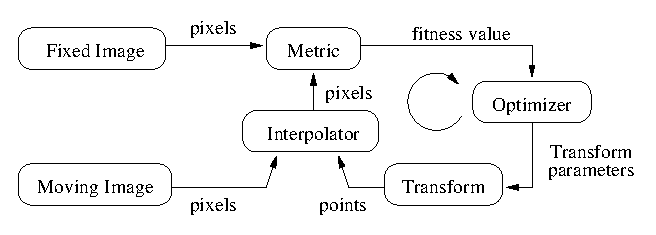
\includegraphics[width=0.8\textwidth]{RegistrationComponentsDiagram.eps}
%\itkcaption[Registration Framework Components]{The basic components of the
%registration framework are two input images, a transform, a metric, an
%interpolator and an optimizer.}
%\label{fig:RegistrationComponents}
%\end{figure}



%%%%%%%%%%%%%%%%%%%%%%%%%%%%%%%%%%%%%%%%%%%%%%%%%%%%%%%%%%
%
%  Example on how to insert an equation.
%  Never forget to put an equation in your paper.
%  They make them look professional and impress the reviewers.
%
%%%%%%%%%%%%%%%%%%%%%%%%%%%%%%%%%%%%%%%%%%%%%%%%%%%%%%%%%%


%To support shape-guidance, the generic level set equation
%(Eqn(~\ref{eqn:ShapeInfluenceTerm})) is extended to incorporate a shape guidance
%term:
%
%\begin{equation}
%\label{eqn:ShapeInfluenceTerm}
%\xi \left(\psi^{*}(\mathbf{x}) - \psi(\mathbf{x})\right)
%\end{equation}




%%%%%%%%%%%%%%%%%%%%%%%%%%%%%%%%%%%%%%%%%
%
%  Insert the bibliography using BibTeX
%
%%%%%%%%%%%%%%%%%%%%%%%%%%%%%%%%%%%%%%%%%

\bibliographystyle{plain}
\bibliography{InsightJournal}


\end{document}
